%%%%%%%%%%%%%%%%%%%%%%%%%%%
%                         %
%       2016.11.16.       %
%      Szakdolgozat       %
%    Tamás     LATEX      %
%%%%%%%%%%%%%%%%%%%%%%%%%%%
\documentclass[oneside,titlepage,12pt,a4paper]{report}
%\documentclass[12pt]{report}
\usepackage[centertags]{amsmath}
\usepackage{amsfonts}
\usepackage{amsthm}
\usepackage{newlfont}
%\usepackage[ansinew]{inputenc}
\usepackage[magyar]{babel}	
\usepackage[utf8]{inputenc}		
\usepackage{t1enc}				
\usepackage{graphicx}
\usepackage{color}
%\usepackage[colorlinks]{hyperref}
%\usepackage[active,new,noold,marker]{xrcs}
\usepackage{euler}
\usepackage{amssymb,latexsym}
\usepackage{amsmath}
\usepackage{graphics}
\usepackage{algorithm} 
%\usepackage{algpseudocode} %ezzel összeakadhat \usepackage{algorithmic} 
\usepackage{rotating}
\usepackage{bigstrut}
\usepackage{subfigure}
\usepackage{appendix}
\usepackage{setspace}


\newtheorem{theorem}{Theorem}
\newtheorem{corollary}{Corollary}
\newtheorem{lemma}{Lemma}
\newtheorem{proposition}{Proposition}
\newtheorem{definition}{Definition}
\newtheorem{notation}{Notation}

\textwidth=6.truein \textheight=9.truein \hoffset=-.5truein
\voffset=-.8truein

\frenchspacing				
\setlength{\parskip}{\smallskipamount}	
\renewcommand{\appendixtocname}{Függelék}
\renewcommand{\appendixpagename}{Függelék}
\DeclareMathOperator{\grad}{grad}
\DeclareMathOperator{\sgn}{sign}
\DeclareMathOperator{\PRD}{PRD}
\DeclareMathOperator{\CR}{CR}
\newcommand{\conj}[1]{\overline{#1}}

\begin{document}
\begin{titlepage}
	\parbox[t]{5.5cm}{\vspace{1cm}}
\begin{center}
	\large
	\textsc{Eötvös Loránd Tudományegyetem \linebreak Informatikai Kar} \\[2cm]
\end{center}

\begin{center}
	% Title
	\LARGE EKG jelek feldolgozása Hermite-függvények segítségével\\[0.55cm]
	\large BSc Szakdolgozat \\[1.9cm]
\end{center}

\begin{center}
	\parbox[t]{25mm}{Készítette:}
	\parbox[t]{5.5cm}
		{Dózsa Tamás\\
		ELTE IK\\
		Programtervező informatikus \\
		BSc
		}
	\\[0.9cm]
	
  \parbox[t]{25mm}{Témavezető:}
	\parbox[t]{5.5cm}{
		Dr. Kovács Péter\\
		Adjunktus\\
		ELTE IK\\
		Numerikus Analízis Tanszék
		}
	\\[4cm]
\end{center}

\begin{center}
	
\includegraphics[scale=0.7]{./Abrak/Egyeb/elte_logo.jpg}\\[1cm]
	Budapest, 2016.11.16.
\end{center}
\end{titlepage}

\tableofcontents

%%%%%%%%%%%%%%%%%%%%%
% BEVEZETES
%%%%%%%%%%%%%%%%%%%%%

\chapter{Bevezetés}
\label{intro}

\par
Az információ ábrázolásának módja az informatika tudomány fontos kérdése. Természetesen annak eldöntése, hogy egy adott adat halmaz milyen módon kerül ábrázolásra erősen függ annak jellegétől. Az adatábrázolás felel az adatok hatékony felhasználhatóságáért (például egy internetes video hívásnál az adatokat gyorsan kell egymás után továbbítani), ugyanakkor biztosítania kell, hogy az adatokból kinyerhető információ nem veszik el (ha túl rossz mindőségű képeket továbbítunk, a fogadó fél nem tudja értelmezni azokat). 
\par	A szakdolgozat célja egy speciális adatábrázolás, nevezetesen EKG jelek egy ábrázolásának bemutatása. Mivel jellemzően ezeket az adatokat, későbbiekben \textit{jelek}-et, általában nagyobb memória felhasználásával szokás ábrázolni, ezért a dolgozat az eljárásra EKG jelek \textit{tömörítéseként} hivatkozik. EKG jelek esetén az ábrázolás minősége sok szemponttól függ. Mivel ezek a jelek fontos információkat hordoznak a szív állapotáról, különösen fontos, hogy a tömörítés során ne vesszen el fontos információ. Egy ilyen jel rögzítésekor azonban sok olyan adat is tárolásra kerül (például a végtagok mérés közbeni mozgatása miatt), amelyek nem hordoznak fontos információt. Az ilyen adatokra a dolgozat \textit{zaj}-ként hivatkozik. Egy jó EKG ábrázolás sikeresen szűri a mérés során keletkezett zajt, miközben az orvosi szempontból fontosnak nevezhető információt megtartja. Mivel a dolgozatban egy tömörítési eljárás kerül bemutatásra, fontos szempont az EKG jelek memória takarékos ábrázolása. Gyakorlati szempontból minél kevesebb memórián történik meg a jelek ábrázolása, annál könnyebb azokat tárolni (hosszú mérések esetén fontos lehet), illetve egyszerűbb és biztonságosabb a jelek hálózaton törtenő továbbítása. EKG jeleknek egy igazán jónak nevezhető ábrázolása pedig az eddig említettek mellett az orvosok munkáját közvetlenül segítő információt is kódol magában. Ilyen lehet például egy olyan ábrázolás amely hatékony bemenetéül szolgál valamilyen osztályozó algoritmusnak, lehetővé téve az abnormális jelek automatikus felismerését. 
	\par A dolgozat három fő fejezetre tagolható. A Bevezetés című fejezetben található a dolgozatban bemutatott eljárás specifikációja, a jel reprezentáció matematikai modelljének ismertetése, valamint a bemutatott módszer egyéb jellemzőit ismertető alfejezetek. Ezek közé tartozik például a jel közelítésének optimalizációjához szükséges Nelder-Mead algoritmus elméleti bemutatása, illetve az EKG jel szegmentációját elősegítő Matching-Pursuit algoritmust részletező alfejezet. 
\par	A dolgozat második fejezete az eljárás mellékelt implementációjának a fejlesztői dokumentációja. Ebben a fejezetben találhatóak a tömörítő eljárást implementáló c++ osztályok jellemzői, illetve az elérést segítő webes felület implementációjának részletes ismertetése. A fejlesztői dokumentáció fejezet tartalmazza továbbá a program logikai jellemzését elősegítő UML és egyéb osztálydiagrammokat. A fejezet igyekszik pragmatikusan és érthetően jellemezni a program felépítését, illetve kellően megindokolni az egyes implementációk mellett szóló döntéseket. 
\par	A Felhasználói dokumentáció fejezetbe, a program használatával kapcsolatos információk kerültek. Ebben a fejezetben található a felhasználói felület funkcióinak pontos ismertetése, valamint hasznos példák annak használatára. Bemutatásra kerülnek továbbá a program használatához szükséges előkészületi lépések, és az ismert rendszerkövetelmények. 
\par	A dolgozat utolsó része a függelék, melyben a Bevezetés fejezetben található matematikai állítások bizonyításai, egyéb kapcsolódó matematikai fogalmak leírásai, illetve felhasznált algoritmusok pszeudo-kódja található. 
		
\section{A feladat specifikációja}

A dolgozat célja egy olyan tömörítési eljárás bemutatása, amely lehetővé teszi az EKG jelek hatékony (memória takarékos) ábrázolását, a mérések zaj szűrését, illetve az EKG hullámszegmenseinek szeparációját. Az utóbbi jellemző orvosi szempontból lehet hasznos, ugyanis sok kóros elváltozás kimutatásához szükséges az egyes hullámszegmensek széleinek ismerete. A dolgozatban bemutatott módszer hatékonysága, az irodalomban fellelhető más tömörítési eljárások \cite{} hatékonyságának összehasonlításával igazolandó. \par A dolgozatban bemutatott tömörítési eljárás implementációjának feladata, hogy az MIT-BIH adatbázisban található EKG jelek tömörítésére alkalmas legyen, ehhez pedig egy könnyen használható webes felületet biztosítson. Az implementációnak két féle bemente megengedett: tömörítés esetén az MIT-BIH adatbázisban megtalálható EKG jelek, illetve a tömörítés következtében létrejött számsorozat, melyet a tömörített jel helyreállításához használ.  

\section{A modell ismertetése}
A modern orvostudományban nagy jelentőséggel bírnak 
a valamely élő szervezet által kibocsátott úgynevezett $biológiai jelek$. Ezek közé sorolható az $Elektro$ $Kardio$ $Gram$, vagy $EKG$,
amely a szív állapotáról képes információt adni. Bár ennek a dolgozatnak nem célja az $EKG$ jelek pontos elemzése, fontos néhány sorban ismertetni egy átlagos $EKG$ jel meghatározó hullámait. Egyetlen szí vütés  $EKG$ reprezentációja három fő részre bontható: a szí vütés elején megjelenő $P$ hullámra, az ezt követő $QRS$ komplexumra, és az ütés végén található $T$ hullámra. Ezek rendre a pitvari összehűzódást, a kamrák depolarizációját és elektromos újratöltődését reprezentálják. Diagnosztikai szempontból a $QRS$ komplexus a legfontosabb, ezért ezt nagy pontossággal kell tárolni. Általánosságban elmondható, hogy ezeknek a hullámoknak kezdő és végpontjai, valamint maximum és minimum értékei vesznek részt az orvosi diagnosztikában. Az említett paraméterek az \ref{fig:ekg} ábrán láthatóak.

\begin{figure}[htb!]
\begin{center}
   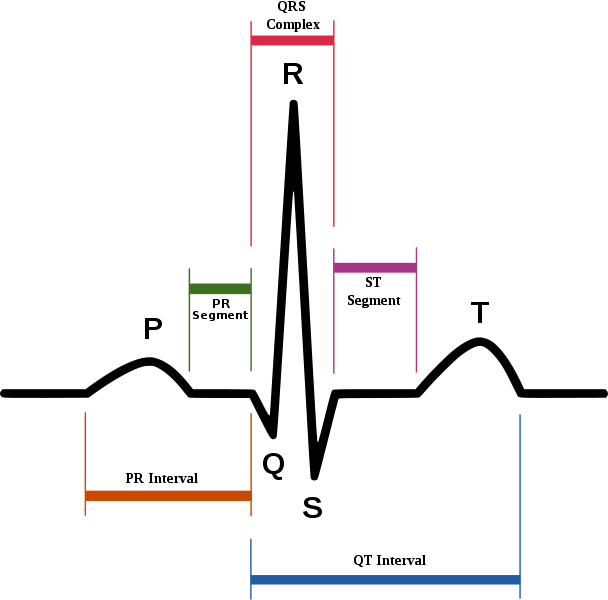
\includegraphics[scale=0.37]{./Abrak/Egyeb/ecg_wiki.png}
   \caption{Az EKG jel egy szívütése, illetve annak főbb diagnosztikai jellemzői.}
		\label{fig:ekg}
\end{center}
\end{figure}
 
Az irodalomban ismert tömörítő algoritmusokat \cite{unifiedReview} alapján három kategóriába sorolhatjuk: 1) egyszerű paraméteres becslések (pl.: interpoláció, különbségi kódolás, stb.), 2) direkt módszerek (pl.: csúcsok, meredekségek, stb. tárolása), 3) transzformációs eljárások. Az utóbbi osztály tartalmazza azokat az algoritmusokat, melyek a jelet egy előre adott függvényrendszer szerinti sorfejtéssel approximálják. Így az eredeti adatsorozat helyett csak az együtthatókat és a rendszer paramétereit kell tárolnunk. Ezen kategóriába sorolandó a dolgozatban bemutatott algoritmus is. Nevezetesen, az eredeti adatsorozatot speciális, Hermite-polinomok segítségével előállitott függvényrendszerrel fogjuk közelíti. A módszer alapját képező eljárás \cite{hexp3}, jól ismert az irodalomban, mely nem csak a jelek tömörítéséhez, de azok modellezéséhez \cite{hexp2}, illetve osztályozásához \cite{hexp1, hexp4} is alkalmazható. A dolgozatban az EKG jelekkel való hasonlóságuk miatt Hermite-függvényeket használunk az adatok reprezentálásához. Ezeket egy argumentum transzformáción keresztül szabad paraméterekkel egészítjük ki. Ennek köszönhetően az eredeti jelet egy adaptív bázisban írhatjuk fel. Az említett paraméterek megválasztásához a Nelder-Mead optimalizációs eljárást alkalmaztuk. Mivel az EKG jelek diszkrét adatsorozatok, ezért a módszert \cite{hexp5} alapján implementáltuk diszkrét ortogonális Hermite-polinomokra is. A dolgozatban különböző tesztekkel demonstráljuk az algoritmus hatékonyságát. Ehhez, több órányi, zajjal terhelt, valódi EKG felvételt használtunk. Ezen keresztül a bemutatott módszert összehasonlítottuk több másik, az irodalomban jól ismert tömörítő algoritmussal is \cite{jpeg2000ECG}. 

A tömörítő eljárást egy c++ nyelven megírt, objektum elvű alkalmazás implementálja, melyet egy webes felületen keresztül érhetünk el. A felület lehetőséget biztosít a dolgozatban jelölt tesztek újrafuttatására, valamint a teszteléskor felhasznált adatbázis további jeleinek a tömörítésére. Szintén a webes felületen keresztül nyílik alkamunk a már tömörített EKG jelek helyreállítására. 

Az alkalmazás megetrvezésekor külön hangsúlyt kapott a kód újra felhasználhatósága. Ennek érdekében a felhasznált algoritmusok, illetve matematikai modellek a lehető legáltalánosabb formában lettek implementálva. Fontos szempontot jelentett továbbá a c++11-es nyelvszabvány által nyújtotta lehetőségek minél hatékonyabb kihasználása. Jó példa erre a lambda függvények alkalmazása az optimalizációs algoritmusok implementációja során. A hatékony működés mellett azonban a program igyekszik megfelelni a modern felhasználók igényeinek. Ennek érdekében a felhaszálói felület weboldalként lett implementálva. A rendszerfüggetlen, és installáció mentes elérés lehetővé teszi a gyors és egyszerű használatot, valamint az eredmények megosztását.  

\section{Matematikai háttér}
\subsection{Jelek approximációja}

EKG jelek feldolgozásakor sok esetben szembesülünk gyakorlati kihívásokkal. Két sűrűn előforduló példa a hosszú mérések tárolása, valamint a zajjal terhelt mérések ábrázolása. Ezekre a nehézségekre egyszerre ad kielégítő megoldást, ha a jeleket  valamely $\mathcal H$ Hilbert-tér sima függvényeiből álló $(\Phi_n, n\in\Bbb N)$ ortogonális bázisában reprezentáljuk és a jelet véges sok $\Phi_0,\Phi_1,\cdots,\Phi_n$ bázisbeli elem lineáris kombinációjával közelítjük. Az $f\in\mathcal H$ jel
legjobb közelítését a tér $\|\cdot\|$ normájában az
$$
S_nf:=\sum_{k=0}^n\langle f,\Phi_k\rangle \Phi_k
$$
leképezés nyújtja, ahol $\langle\cdot,\cdot\rangle$ az $\mathcal  H$ tér
skaláris szorzatát jelöli. A jel és a közelítés eltérésének négyzete  a
$$
\|f-S_nf\|^2=\|f\|^2-\sum_{k=0}^n|\langle f,\Phi_k\rangle|^2
$$
képplettel adható meg. Adott hibán belüli közelítést véve a jel helyett  elég az
$S_nf$ approximációt reprezentáló  $\langle f,\Phi_k\rangle\ (k=0,1,\cdots, n)$ Fourier-együtthatókat tárolni.  Zajos jel esetén az ilyen típusú approximáció szűrőként is szolgál.  A közelítés megvalósításához a klasszikus ortogonális rendszerek közül  EKG görbék közelítésére  az Hermite-féle függvények bizonyultak használhatónak. Ezt támasztják alá a [...] dolgozatok. Az  Hermite függvények alkalmazása azzal is indikolható, hogy grafikonjuk hasonlít az EKG görbékre. Ezt a tulajdonságot a \ref{fig:phi0-3} ábra szemlélteti.

%\begin{figure}
%  \centering
%\subfigure[$\Phi_{0}(x)$]{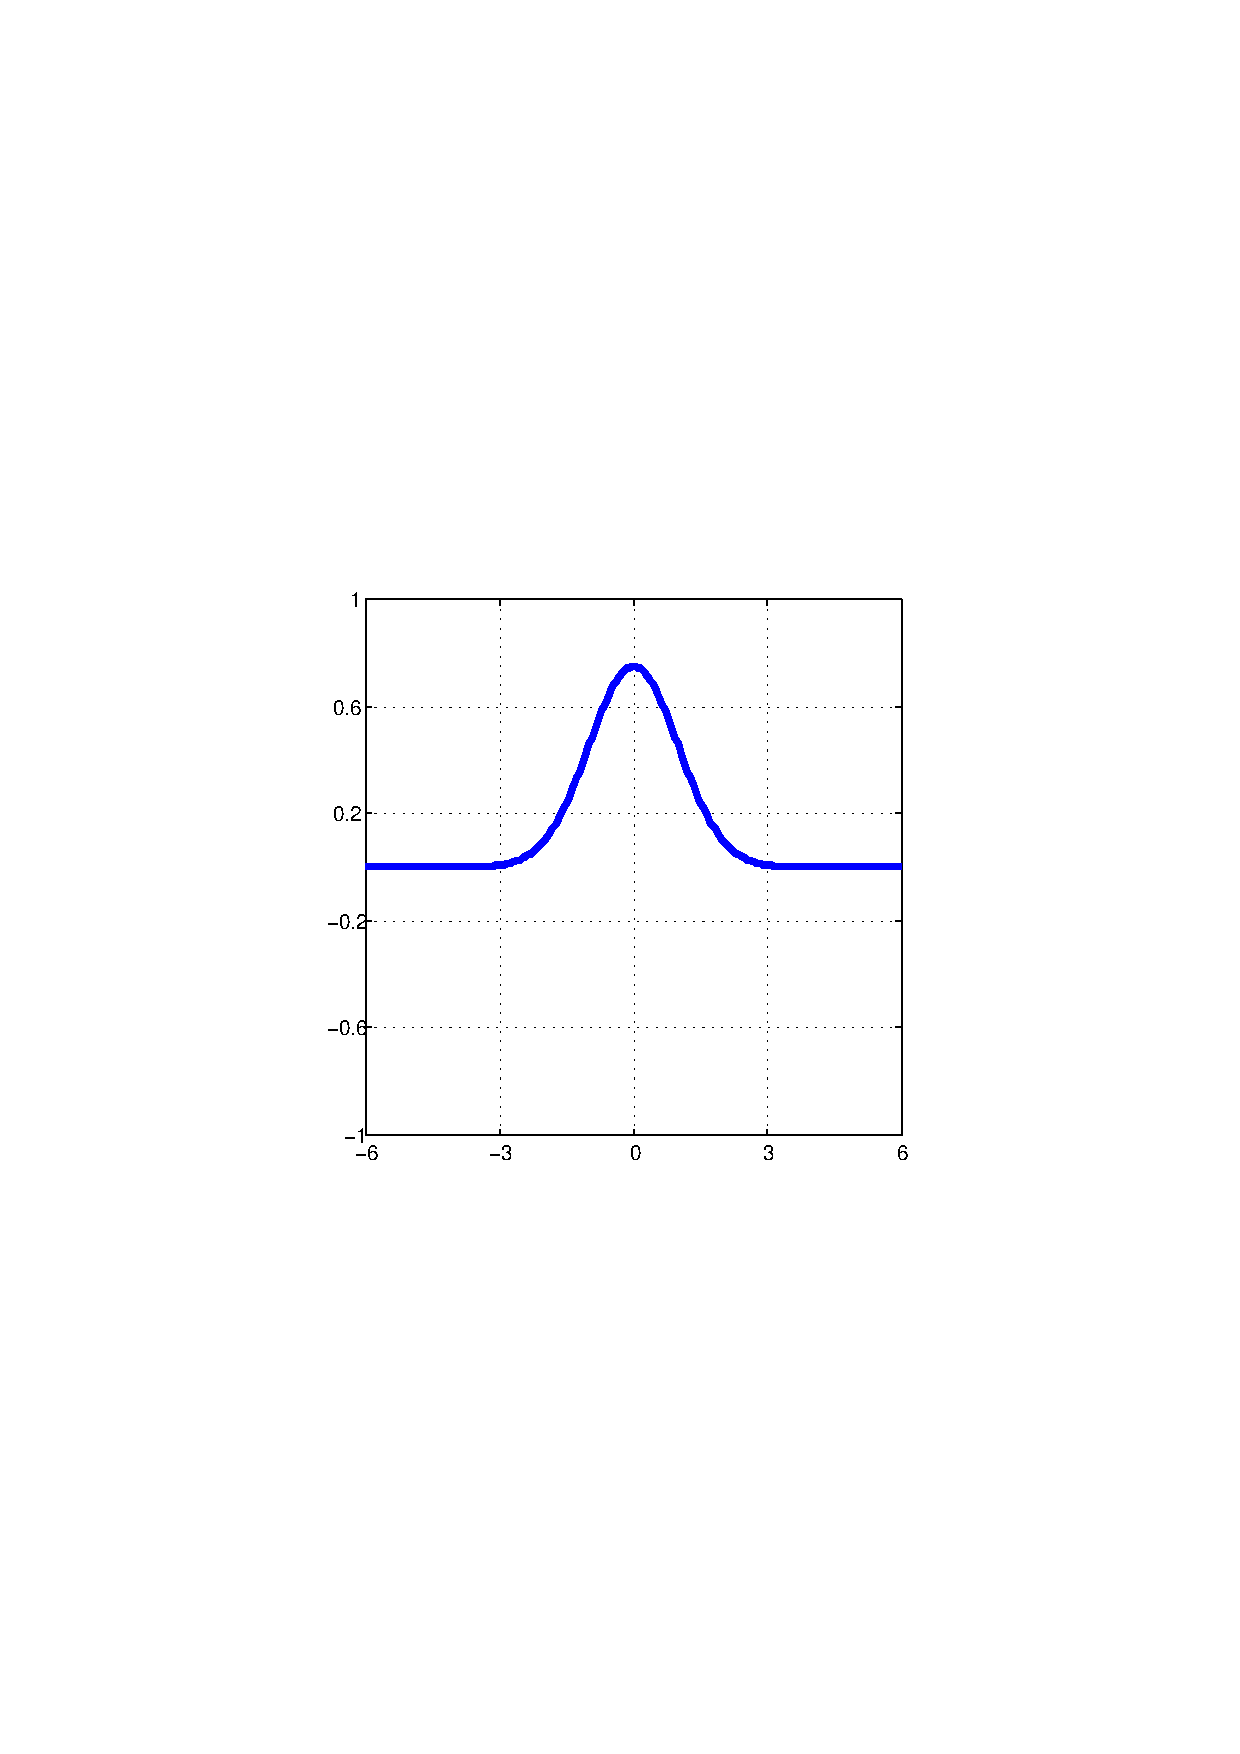
\includegraphics[scale=0.34,trim=150 280 150 280,clip]{./%Abrak/Egyeb/phi0.pdf}} 
%\subfigure[$\Phi_{1}(x)$]{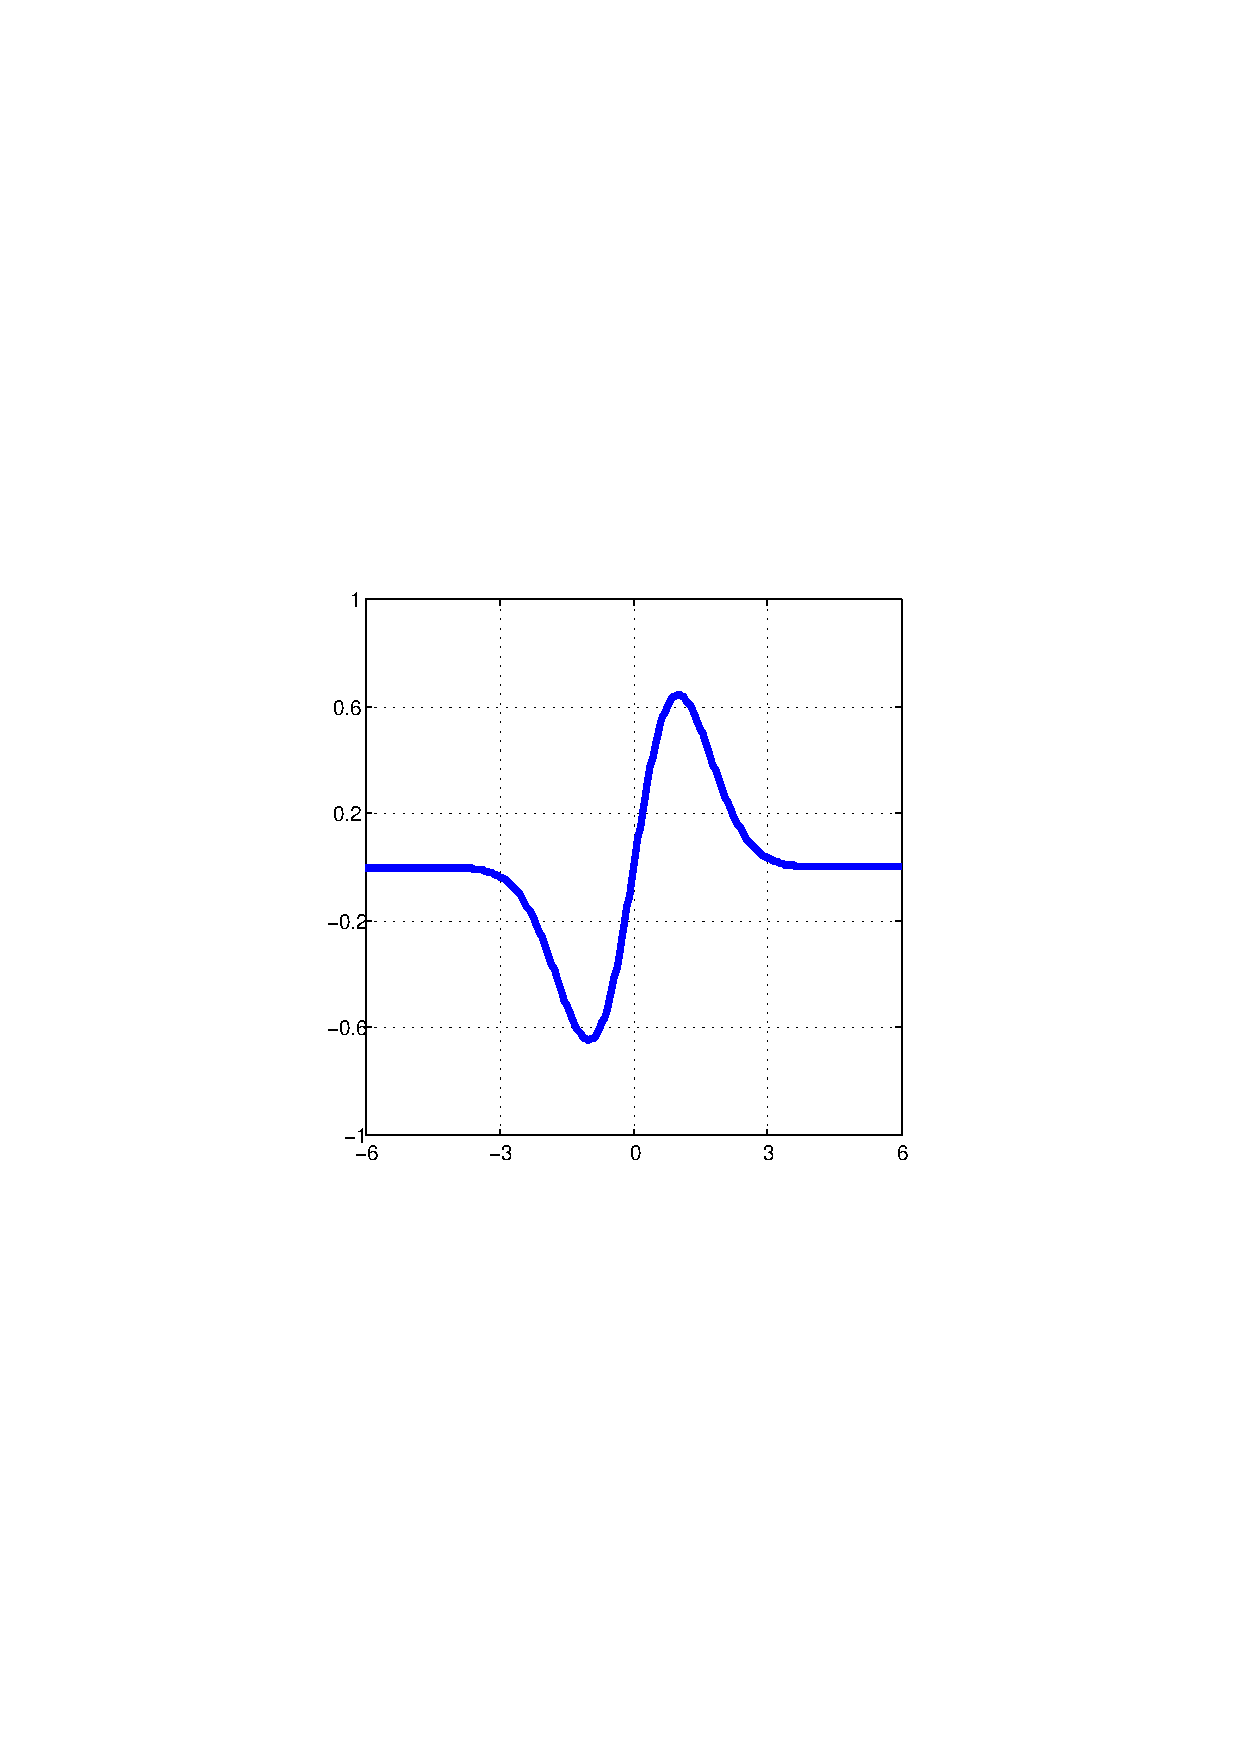
\includegraphics[scale=0.34,trim=150 280 150 280,clip]{./%Abrak/Egyeb/phi1.pdf}}
%\subfigure[$\Phi_{2}(x)$]{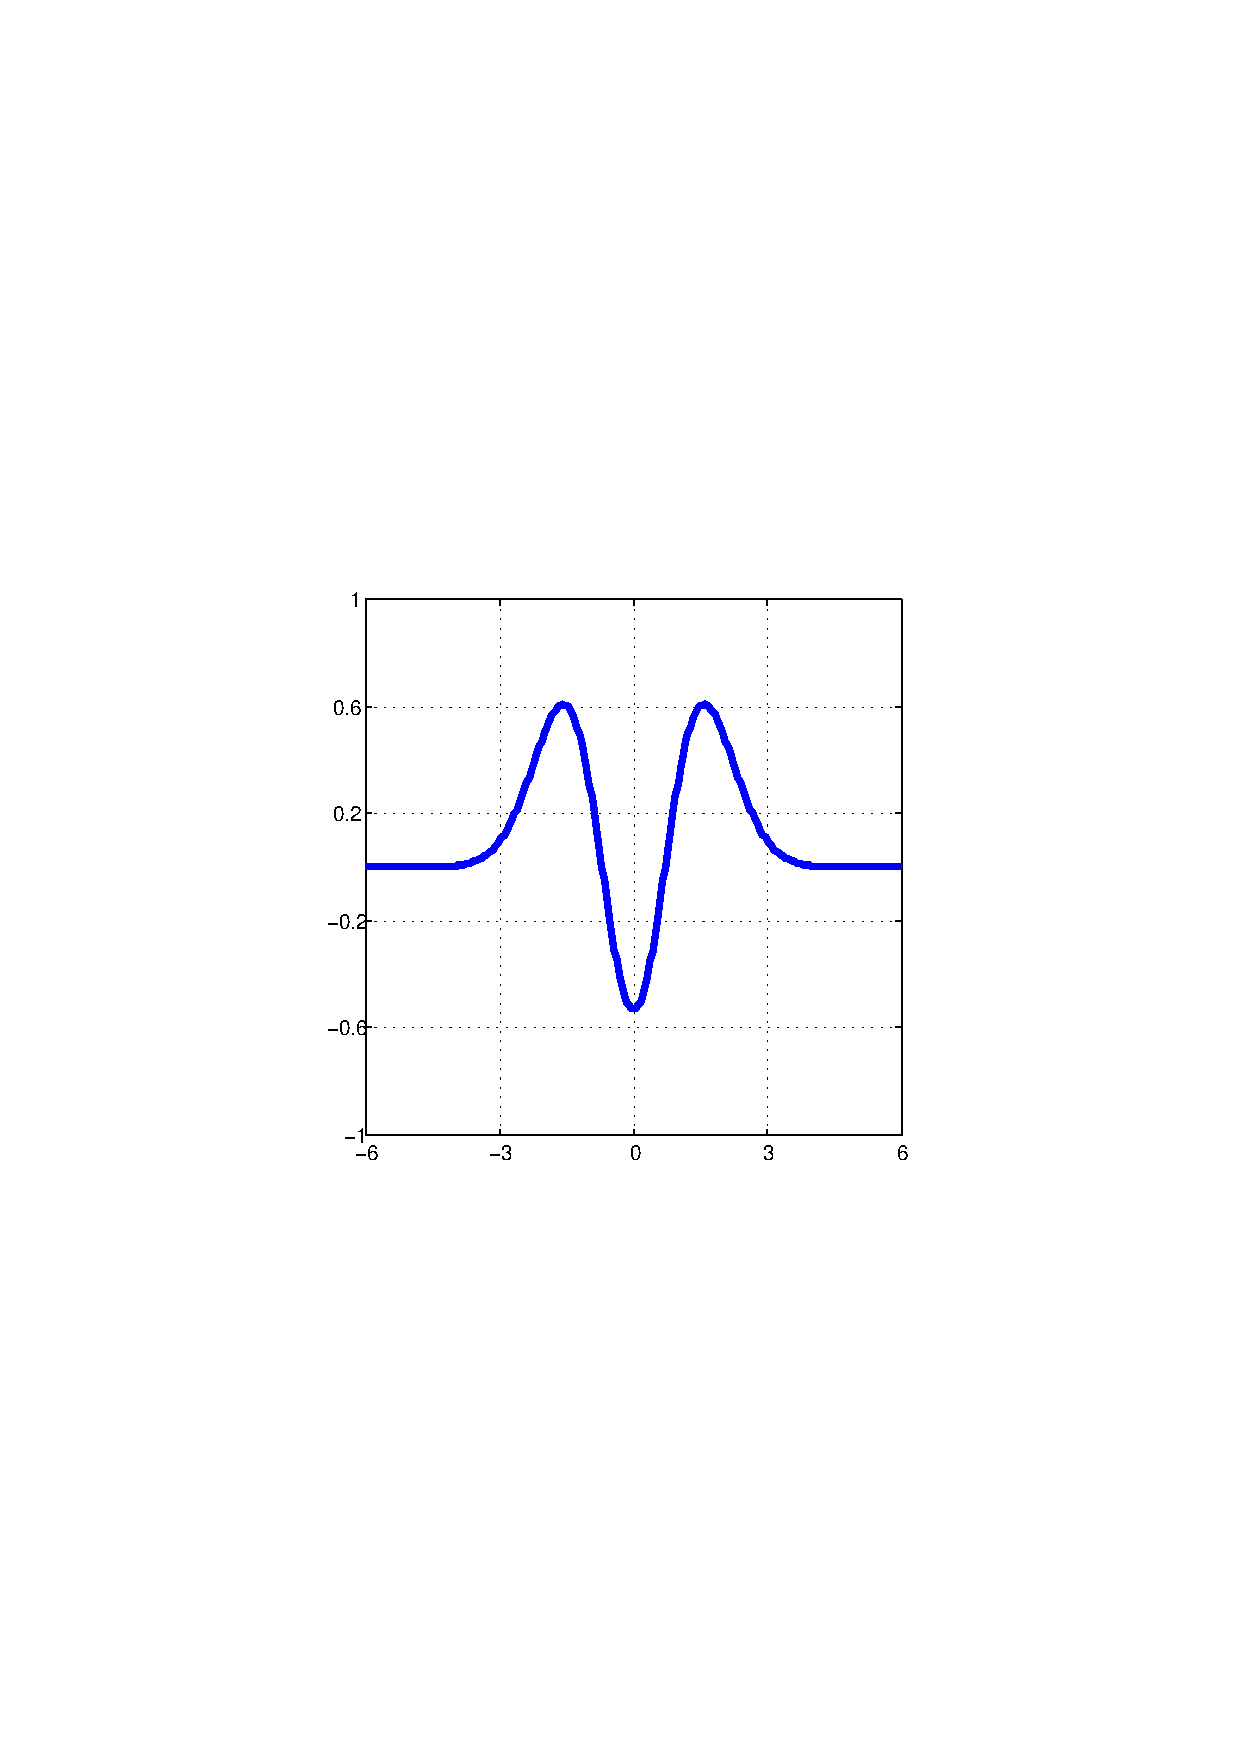
\includegraphics[scale=0.34,trim=150 280 150 280,clip]{./%Abrak/Egyeb/phi2.pdf}} 
%\subfigure[$\Phi_{3}(x)$]{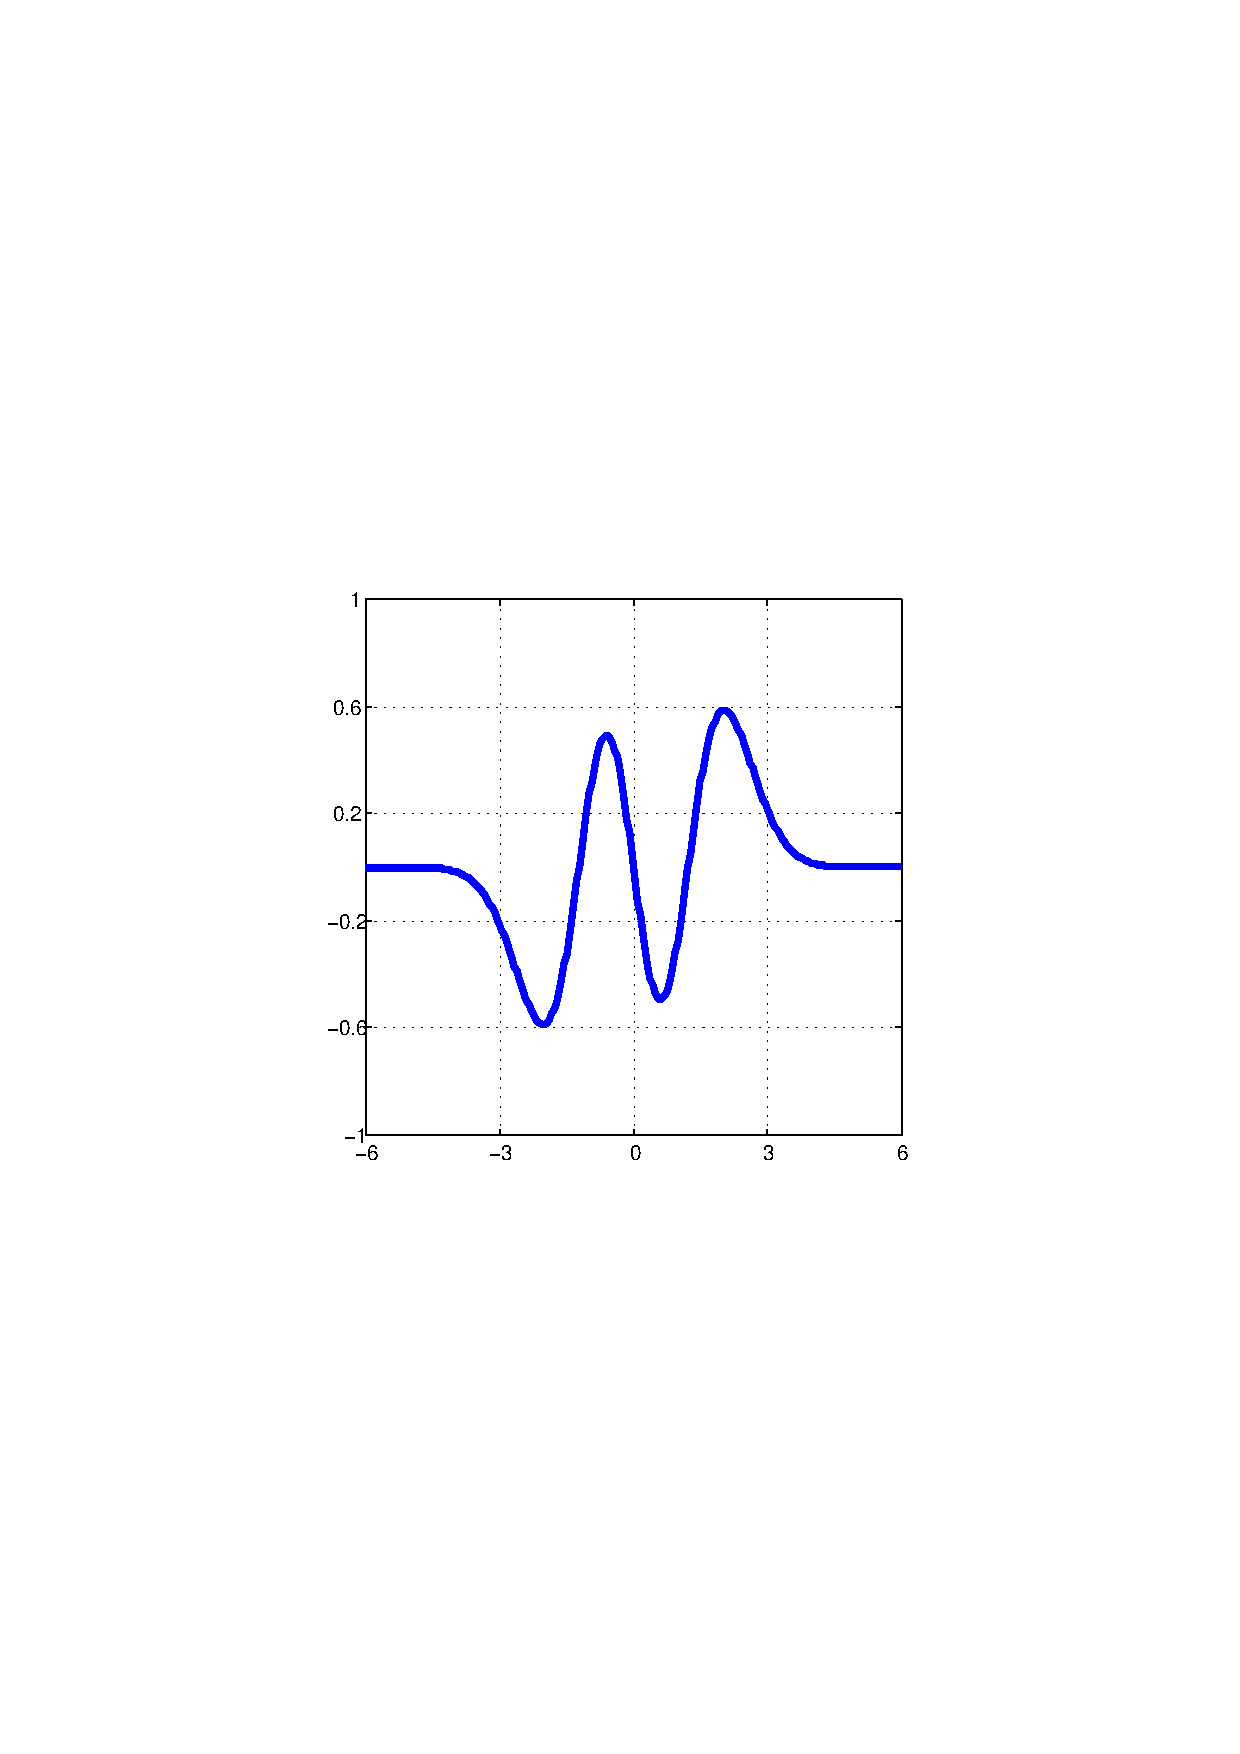
\includegraphics[scale=0.34,trim=150 280 150 280,clip]{./%Abrak/Egyeb/phi3.pdf}}
%\caption{A Hermite-függvényrendszer első négy tagja.}
%\label{fig:phi0-3}
%\end{figure}

\subsection{Hermite-függvények}
A dolgozatban  az $\Bbb R$ számegyenesen (Lebesgue-mérték szerint) négyzetesen integrálható függvények $\mathcal H$ Hilbert-tere helyett elegendő a szakaszonként folytonos, az $\Bbb R$-en  négyzetesen integrálható függvények $\mathcal F$ euklideszi terét használni. Ebben a térben a skaláris szorzat és a norma a következő alakban írható fel:
\begin{equation}
 \langle f,g\rangle:=\int_{-\infty}^\infty f(t)g(t)\, dt,\ \ \|f\|:=\sqrt{\langle f,f\rangle}\ \ (f,g\in\mathcal F)\,.
\label{eq:dotprod}
\end{equation}
Továbbá, a
 \begin{equation*}
 \Phi_n(x):=H_n(x)e^{-x^2/2}/\sqrt{\pi^{1/2}2^n n!}\quad \ (n\in\Bbb N)
 \end{equation*}
normált Hermite-függvények (teljes) ortonormált rendszert alkotnak az $\mathcal F$ téren:
  \begin{equation*}
   \langle \Phi_n,\Phi_m\rangle=\delta_{nm}\ \ (m,n\in\Bbb N),\quad
  \|f-S_nf\|\to 0\ (n\to\infty)\,.
   \end{equation*}
Itt $H_n\ (n\in\Bbb N)$ jelöli az Hermite-féle polinomokat.
\\
\\
Az Hermite-függvények alkalmazásának számos előnye van: \\
\\
i) A $\Phi_n\ (n\in\Bbb N)$ rendszer zárt (teljes) az $\mathcal F$ téren. \\
\\
ii) A $\Phi_n(x)$ függvények gyorsan tartanak $0$-hoz, ha $|x|\to \infty$: \\
$$
|\Phi_n(x)|\le M_n e^{-x^2/4}\le M_n\ \ (x\in\Bbb R, n\in\Bbb N).
$$
\\
iii) A $\Phi_n$ függvények (stabil) másodrendű rekurzióval számíthatók: \\
\begin{equation}
\begin{split}
&\Phi_0(x):=e^{-x^2/2}/\pi^{1/4},\ \Phi_1(x):=\sqrt{2}\, x e^{-x^2/2}/\pi^{1/4}\\
&\Phi_n(x)=\sqrt{\frac 2 n} x \Phi_{n-1}(x)-\sqrt{\frac{n-1}n}\Phi_{n-2}(x)\ \ (x\in\Bbb R, n\ge 2)
\end{split}
\end{equation} 
\\
\\
iv) A $\Phi_n'$ deriváltak kifejezhetők a $\Phi_n, \Phi_{n-1} $ függvényekkel: \\
\begin{equation}
\Phi_n'(x)=\sqrt{2n}\Phi_{n-1}(x)-x\Phi_n(x)\ \ (x\in\Bbb R, n\in\Bbb N,\Phi_{-1}=0)
\end{equation}

\subsection{Az approximáció optimalizálása}

A jelek reprezentációja  függ az időskála $0$ pontjának és az egység
megválasztásától. Ezeket a paramétereket  a gyakorlatban önkényesen szoktuk
 megválasztani. Ezzel összefüggében felvethető a kérdés, hogyan lehet optimálisan megválaszthatani  ezeket a paramétereket.
Az  approximáció pontossága javítható azonos együttható szám mellett, amennyiben az  Hermite-függvények helyett azok
\begin{equation}
\Phi_n^{a,\lambda}(x):=\Phi_n(\lambda x+a)\ \  (x,a\in\Bbb R, \lambda>0)
\end{equation}
affin transzformáltjait használjuk. A $\sqrt{\lambda}\Phi_n^{a,\lambda}\ (n\in\Bbb N)$ rendszer is ortonormált és teljes az $\mathcal F$ téren. Ebben az esetben
az $f$ legjobb approximációja az
\begin{equation}
S_n^{a,\lambda}f:=\sum_{k=0}^n\langle f,\Phi_k^{a,\lambda}\rangle\Phi_k^{a,\lambda}\ \
(n\in\Bbb N, a\in\Bbb R,\lambda>0)
\end{equation}
projekció és a közelítés hibája az $a$ transzlációs és a $\lambda$ dilatációs paraméter függvénye:
\begin{equation}
D^2_n(a,\lambda):=\|f\|^2-\sum_{k=0}^n|\langle f,\Phi_k^{a,\lambda}\rangle|^2.
\end{equation}
            E két szabad paraméter optimalizálásával azonos együtthatószám mellett, az eredeti Hermite polinomokkal törtánő  approximációhoz képest pontosabb közelítés érhető el. A $D_n$ függvény minimalizálása ekvivalens  az
 $$
 F_n(a,\lambda):=\sum_{k=0}^n|\langle f,\Phi_k^{a,\lambda}\rangle|^2
 $$
 függvény maximumának meghatározásával. A paraméteres integrálok tulajdonságaiból következik, hogy az
 $$
 A_n(a,\lambda):=\langle f,\Phi_k^{a,\lambda}\rangle \ \  ((a,\lambda)\in T:=\Bbb R\times (0,\infty))
 $$
 Fourier-együtthatók a $T$ tartományon a paraméterek sima függvényei. Bebizonyítható, hogy $\lambda\to 0$ és $|a|+\lambda\to \infty$ esetén
 $F_k(a,\lambda)\to 0$, következésképpen az $F_n$ függvénynek létezik a
 maximuma és a $D_n$ függvénynek létezik a minimuma. A részleteket a Függelékben találhatók.

 Az alábbi ábrák az $F_n(a,\lambda)$ függvényeket szemléltetik fényintenzitás és perspektivikus ábrázolást használva. A harmadik ablakon
a jel közelí tését szemlélteti a maximum helynek megfelelő, ill.  egyéb
paraméter esetén.

\begin{figure}[H]
\begin{center}
   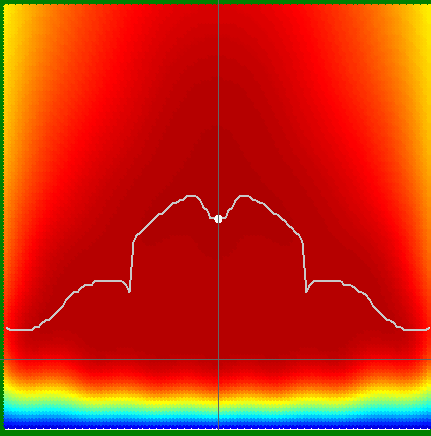
\includegraphics[width=100mm]{./Abrak/Ereszkedo1/F_2sz.png}
  \caption{Az $F_n$ szí nkódos ábrázolása}
\end{center}
\end{figure}

\begin{figure}[H]
\begin{center}
   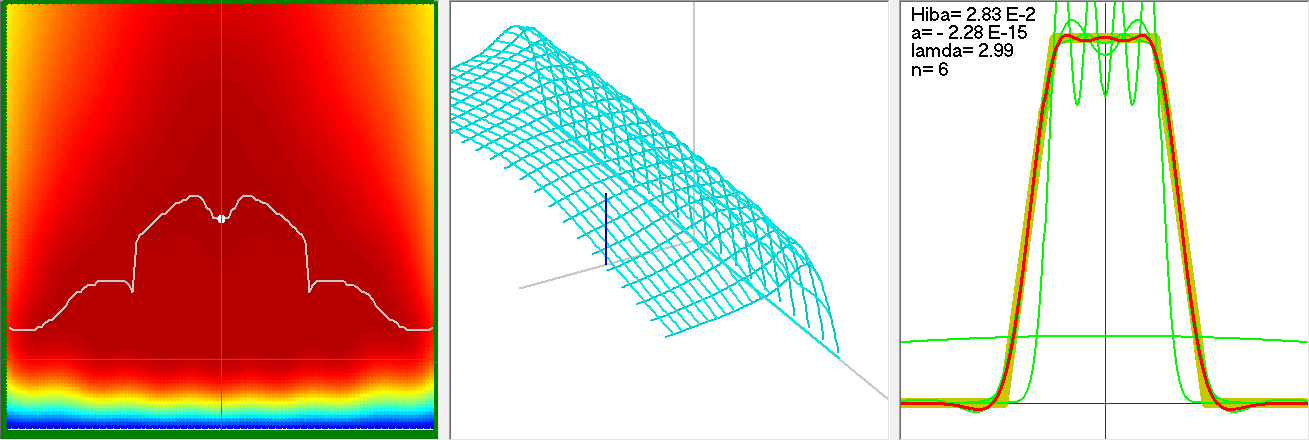
\includegraphics[width=140mm]{./Abrak/Ereszkedo1/Er36.png}
  \caption{Az $F_n$ által meghatározott felület, és approximáció}
\end{center}
\end{figure}

\section{A Nelder-Mead algoritmus}

A $Nelder-Mead$ szimplex algoritmust \cite{} eredetileg 1965-ben
fejlesztették ki azzal céllal, hogy létrehozzanak egy eljárást, amely
képes meghatározni egy $f : \Bbb R^n \to \Bbb R$ nemlineáris függvény minimum (maximum) helyét a  gradiens felhasználása  nélkül, pusztán a függvényértékekre  támszkodva.
Mivel az algoritmust kétváltozós függvényekre alkalmazzuk, ezért ebben a speciális esetben szemléltetjük, megjegyezve, hogy hasonló elvek szerint
 működik az általános $n$ dimenziós eset is. A minimum meghatározásához az $f(x_1), f(x_2), f(x_3)$  függvényértékekből indulunk ki, melyek közül egyet lecserélünk az adott lépésben. Nevezetesen, 
\begin{equation*}
f(x_3)\le f(x_2)\le f(x_1)
\end{equation*}
 esetén olyan $x'$ helyet keresünk, amelyre $f(x')\le  f(x_3)\le f(x_2)$ teljesül és az $x_3, x_2, x_1$ ponthármasról az $x_1$-et elhagyva áttérünk az $x',x_3, x_2$ hármasra. Az $x'$ pontot az előzőekből geometriai transzformációkkal származtatjuk, felhasználva az  $x_2x_3$ szakasz $x=(x_2+x_3)/2$ felezéspontját: 
\begin{equation*}
x'=x_1+\alpha (x-x_1) \quad (\alpha\in\Bbb R)\,.
\end{equation*}
 Az alábbi ábrákon szemléltetjük az algoritmusban  használt transzformációkat. Vegyük észre, hogy $\alpha=2$ esetén $x'$ éppen az $x_1$ pont $x$-re vonatkozó középpontos tükrözése $(T_1).$ Továbbá $\alpha>2$ az eredeti háromszög tükrÖzése + nyújtása $(T_2),$ az $1<\alpha<2$ pedig tükrÖzéses + zsugorításnak felel meg $(T_3).$ A $-1<\alpha<0$ paraméterrel egyszerű zsugorítást kapunk. Végül az 5. transzformáció $(T_5)$ az $x_3$ pontból történő
 kicsinyítésnek feleltethető meg. Az $x_1$ képét ezekben a transzformációkban és a hozzá tartozó függvényértékeket a következő alakban adjuk meg:
\begin{equation*}
x':=x_{3+i}=T_i(x_1)\quad (i=1,2,3,4), \qquad y_j=f(x_j)\quad (j=1,2,\cdots,7)\,.
\end{equation*}
Azt, hogy mikor melyik transzformációt használjuk a Függelékben
található  folyamatábrából látható. Az említett műveleteket a \ref{fig:nmtrf} ábrán szemléltettük.
\begin{figure}[htb!]
  \centering
\subfigure[Tükrözés\ $(T_1: \alpha=2).$]{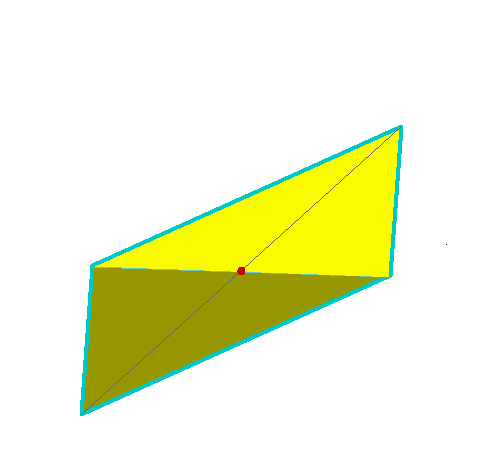
\includegraphics[scale=0.26,trim=10 0 10 53,clip]{./Abrak/Egyeb/NMT1.PNG}} 
\subfigure[T-Nyújtás\ $(T_2: \alpha=2.5).$]{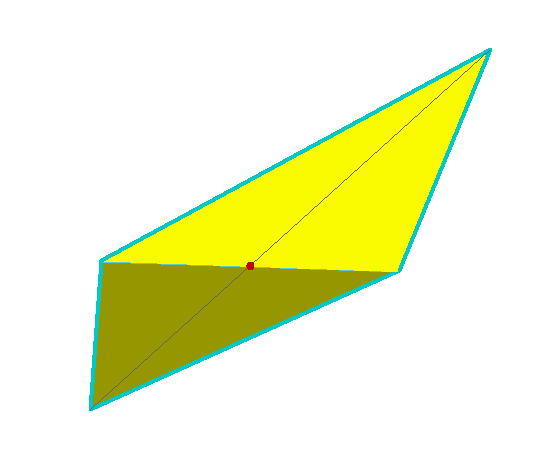
\includegraphics[scale=0.26,trim=10 0 10 53,clip]{./Abrak/Egyeb/NMT2.PNG}}
\subfigure[T-Összehúzás\  $(T_3:  \alpha=1.5).$]{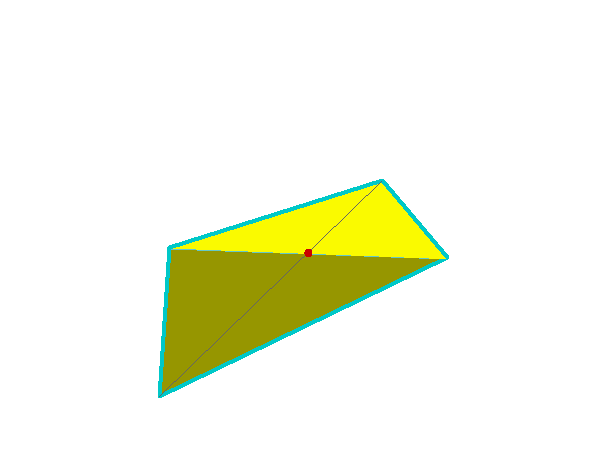
\includegraphics[scale=0.26,trim=10 0 10 53,clip]{./Abrak/Egyeb/NMT3.PNG}} 
\subfigure[Összehúzás\ $(T_4: -1<\alpha<0).$]{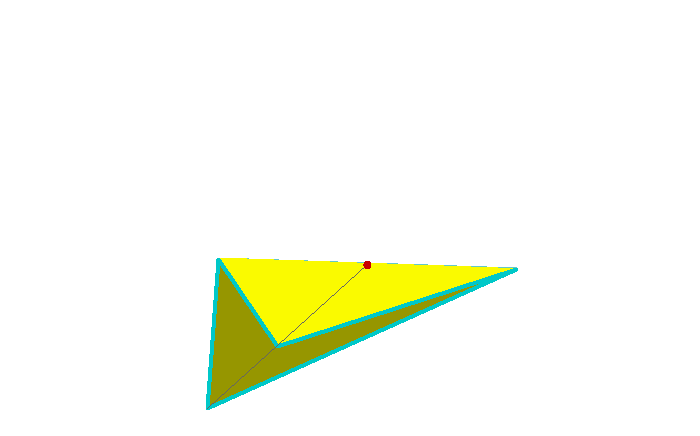
\includegraphics[scale=0.26,trim=10 0 10 185,clip]{./Abrak/Egyeb/NMT4.PNG}}
\subfigure[Kicsinyítés  $x_3$-ból $(T_5).$]{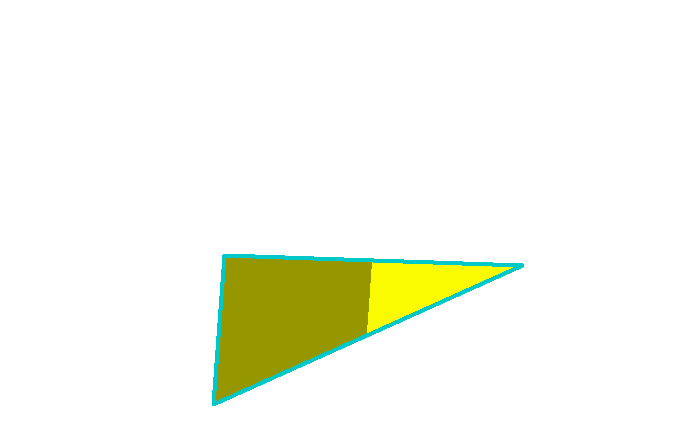
\includegraphics[scale=0.26,trim=10 0 10 185,clip]{./Abrak/Egyeb/NMT5.PNG}}
\caption{A $Nelder-Mead$ szimplex transzformációi.}
\label{fig:nmtrf}
\end{figure}

Megjegyezendő, hogy a $Nelder-Mead$ szimplex módszer is egy determinisztikus algoritmus. Az algoritmus gyors, hiszen minden lépésben csak néhány függvénykiértékelést kell végezni. Továbbá, a gradiens módszerrel ellentétben az olyan patologikus függvények optimumát is képes gyorsan megtalálni, mint amilyen a Rosenbrock függvény. 


\section{Kvadratúra formulák}

Mivel a $Nelder-Mead$, illetve a $PSO$ algoritmusok
csak a függvényértékekre támaszkodnak, a hibafüggvény értékeinek kiszámításához elegendő az Hermite-függvényeket valamilyen felosztás pontjaiban egyszer meghatatározni. Ez implementációs szempontból is fontos, hiszen nem kell minden $(\lambda,a)$ paraméterhez kiszámolni az ettől függő, rekurzióval adott Hermite-féle függvényrendszer tagjait. Ehelyett elég az eredeti diszkrét adatsorozatot dilatálni, illetve eltolni, ami lényegesen kevesebb számítást igényel. Továbbá, az említett felosztás pontjainak valamely Hermite-függvény zérushelyeit választva, a hibafüggvényben  szereplő integrálok kiszámításához
a \cite{waveletECG} dolgozatban használt eljáráshoz hasonlóan kvadratúra formulát is alkalmazhatunk. Ennek előnye, hogy az alappontokban a módszer interpolál, így itt lehetséges a jel mintáinak pontos rekonstrukciója. Ugyanakkor, a kapott approximáció is pontosabb, amit a \cite{waveletECG}-ben közölt numerikus tesztek is alátámasztanak.
	\par Mivel a leggyosrabb ereszkedés módszerének az alkalmazásához 
szükségünk van a függvény parciális deriváltjaira, így ezek előállításával
külön  kell foglalkozni. Az Hermite-függvények deriváltjaira vonatkozó formulák alapján a
parciális deriváltakra a hibafüggvényhez hasonló ellőállítás adható. Ebben az esetben az \eqref{eq:dotprod} egyenletben szereplő integrálok kiszámításához ekvidisztans felosztást alkalmaztunk.


\section{A tömörítő eljárás jellemzése}

	Mindhárom optimalizáció esetén, a tömörítő
eljárás előkészítése megegyezik. A program indításakor az első feladat,
hogy a teljes EKG jelet szívütésekre bontsunk, majd
minden szívütést paraméterként adjunk tovább a tömörítő eljárásnak. Inicializálni kell továbbá
a tömörítő függvények által visszaadott, az aktuális szívütésre vonatkozó Fourier-együtthatókat, 
az approximáció hibáját, illetve az optimalizációs eljárások által meghatározott dilatációs és 
transzlációs paramétereket tároló tömböket. \par
	
A tömörítés előkészítése nem ér véget a jel szívütésekre történő felbontásakor. A szívütéseket normalizáljuk is. Ez azt jelenti, hogy az első és utolsó helyen felvett értékeket összekötő egyenest kivonjuk a jelből. Ezt az eljárást az irodalomban az alapvonal eliminálásnak nevezik. Ennek eredményeként a jel tartója a kezdő és a végpont által meghatározott intervallum. Végül, a szívütést normáljuk, vagyis az egyes értékeket 
elosztjuk az abszolút maximummal. \par
	A tömörítés megkezdése előtt inicializáljuk a függvényrendszert, 
melynek során az egyes bázisfüggvények által felvett értékek egy mátrix soraiba kerülnek: 
\begin{equation*}
	\Phi:=\left[\Phi_n(\alpha_m)\right]_{0\leq n < N,\;0\leq m < M}\,.
	\label{eq:phi_matrix}
\end{equation*}
A $\Phi\in\mathbb{R}^{N\times M}$ mátrix segítségével az $f\in\mathbb{R}^M$ diszkrét jel Fourier-együtthatói könnyen meghatározhatók:
\begin{equation*}
	c_n:=\left\langle f, \Phi_n \right\rangle=\frac{1}{M} \Lambda^{-1} \Phi f \quad (0\leq n < N)\,,
	\label{eq:phi_coeffs}
\end{equation*}
ahol $\mathbb{R}^{N\times N}\ni\Lambda=\Phi \Phi^T$ Cristoffel-Darboux számokat tartalmazza. Az előállításban szereplő $\alpha_n\in\mathbb{R}\, (0\leq n < N)$ számokat a \ref{sec:kvad} fejezetnek megfelelően kétféleképpen határoztuk meg. Egyrészt a $PSO$ és $Nelder-Mead$ algoritmusokban a $\Phi_N$ függvény gyökeit véve kvadratúra formulákat definiáltunk. Másrészt a gradiens módszerhez $f$ tartóján egyenletes alapponterndszert használtunk. Felhívjuk a figyelmet arra, hogy az előbbi esetben a gyökök pontos meghatározása kritikus a feladat szempontjából. A probléma megoldásához a \cite{gautschi} könyv által javasolt numerikus eljárást követjük. Nevezetesen, a $H_n$ Hermite-polinom \eqref{eq:identities} rekurziójában szereplő együtthatókat egy tridiagonális mátrixba rendezzük. Könnyen belátható, hogy az $\alpha_n$ gyökök megegyeznek ezen tridiagonális mátrix sajátértékeivel.  \par

Hátra van még a megfelelő $(a,\lambda)$ paraméterek beállítása. Annak érdekében, hogy a reprezentáció minél adaptívabb legyen, több  optimális transzlációt, illetve dilatációt fogunk meghatározni. Az eredeti $f\in\mathcal{F}$ jelet tehát a következő alakban közelítjük:
\begin{equation*}
	S_{\mathbf{n}}^{\mathbf{a},\boldsymbol{\lambda}}f:=\sum_{i=1}^N\sum_{k=0}^{n_i} \langle f^{a_i,\lambda_i},\Phi_{k}\rangle\Phi_{k} \quad
	(a_k \in \Bbb R,\lambda_k>0)\,,
\end{equation*}
ahol $\mathbf{a}=a_1, a_2, \ldots, a_N$ az alkalmazott transzlációk, $\boldsymbol{\lambda}=\lambda_1, \lambda_2, \ldots, \lambda_N$ pedig a dilatációk sorozata. Az egyes sorfejtésekhez tartozó együtthatók számát az $\mathbf{n}=n_1, n_2, \ldots, n_N$ vektor jelöli. Mivel az EKG jel alapvetően három fő hullámból áll ezért esetünkben $N=3.$ Továbbá a \cite{hexp3} dolgozat eredményei alapján
a QRS komplexumot egy heted, a T hullámot hatod, a P hullámot pedig egy másodfokú ortogonális rendszer segítségével approximáljuk azaz $\mathbf{n}=7,6,2\,.$ Felhívjuk a figyelmet, hogy a legjobb approximáció előállításához a \eqref{eq:hilaprx} egyenlettel ellentétben már az eredeti függvény $f^{a_i,\lambda_i}$ transzformáltját használjuk. Ez nem jelent megszorítást az eredeti problémára nézve, implementációs szempontból viszont $f^{a_i,\lambda_i}$ kiszámítása gyorsabb, mint a $\Phi_n^{a_i,\lambda_i}$ rendszer előállítása.

A $(a_i,\lambda_i)$ paraméter párok optimalizációját egymástól függetlenül végezzük. Így azonban nem garantált, hogy az algoritmus a P, QRS, T hullámokat külön-külön approximálja. A probléma megoldására az irodalomban jól ismert ún. $Matching\ Pursuit$ $(MP)$ konstrukciót \cite{mpurs} alkalmazzuk. Ez egy mohó algoritmus, mely minden lépésben a \eqref{eq:Fnfuggv} egyenletben definiált $F_n(a_i,\lambda_i)$ függvény maximalizálására törekszik. Az iteráció $i.$ lépése a következő alakban írható fel:
\begin{equation}
	s^{(i)}=s^{(i-1)} + S^{a_i,\lambda_i}_{n_i} R^{(i-1)} \quad (1\leq i \leq N)\,,
\label{eq:mpurs}
\end{equation}
ahol $R^{(i)}=f-s^{(i)}$ a rezidum függvényt jelöli. Röviden tehát az $s^{(0)}=0,\ R^{(0)}=f$ inicializálás után, az eljárás $i.$ lépésében megkeressük az $R^{(i-1)}$ függvény $\ell^2$ norma szerinti legjobb közelítését, amit ki is vonunk az említett rezidum vektorból. Ezt $N$ iteráción keresztül ismételjük az aktuális $R^{(i)}$ függvényre. Az MP módszer egy gyors algoritmus, mellyel megkonstruálható az $f\in\mathcal{F}$ jel ritka reprezentációja. Emellett lehetséges az EKG szívütéseinek automatikus szeparációja is, hiszen a jel különböző részeit eltérő ortogonális rendszerek segítségével közelítjük. Felhívjuk a figyelmet arra, hogy az eredeti \cite{hexp3} módszerben ezt a lépést egy külön szegmentáló algoritmus végezte. Így a közelítés pontossága erősen függött a szegmentálás eredményétől (lsd. \ref{sec:test} fejezet). A kifejlesztett eljárásnál azonban ez a probléma nem áll fenn még zajos jelek esetén sem. A dolgozatban bemutatott módszer iterációs lépéseit, az $R^{(i)}$ rezidum függvények alakulását, illetve a szeparált EKG jelet az \ref{fig:mpstep} ábra szemlélteti. Jól látható az is, hogy a fekete vonallal jelölt optimális transzláció általában nem az abszolút maximum helyén található. Ez indokolja, hogy a $\lambda_i$ dilatáció mellett az $a_i$ paraméter optimalizációjára is szükség van. Mivel ez utóbbi a kindulásként használt \cite{hexp3} dolgozatból hiányzik, ezért a pontosság és tömörítési arány jelentős javulását várjuk.
\begin{figure}[htb!]
  \centering
\subfigure[A QRS approximációja.]{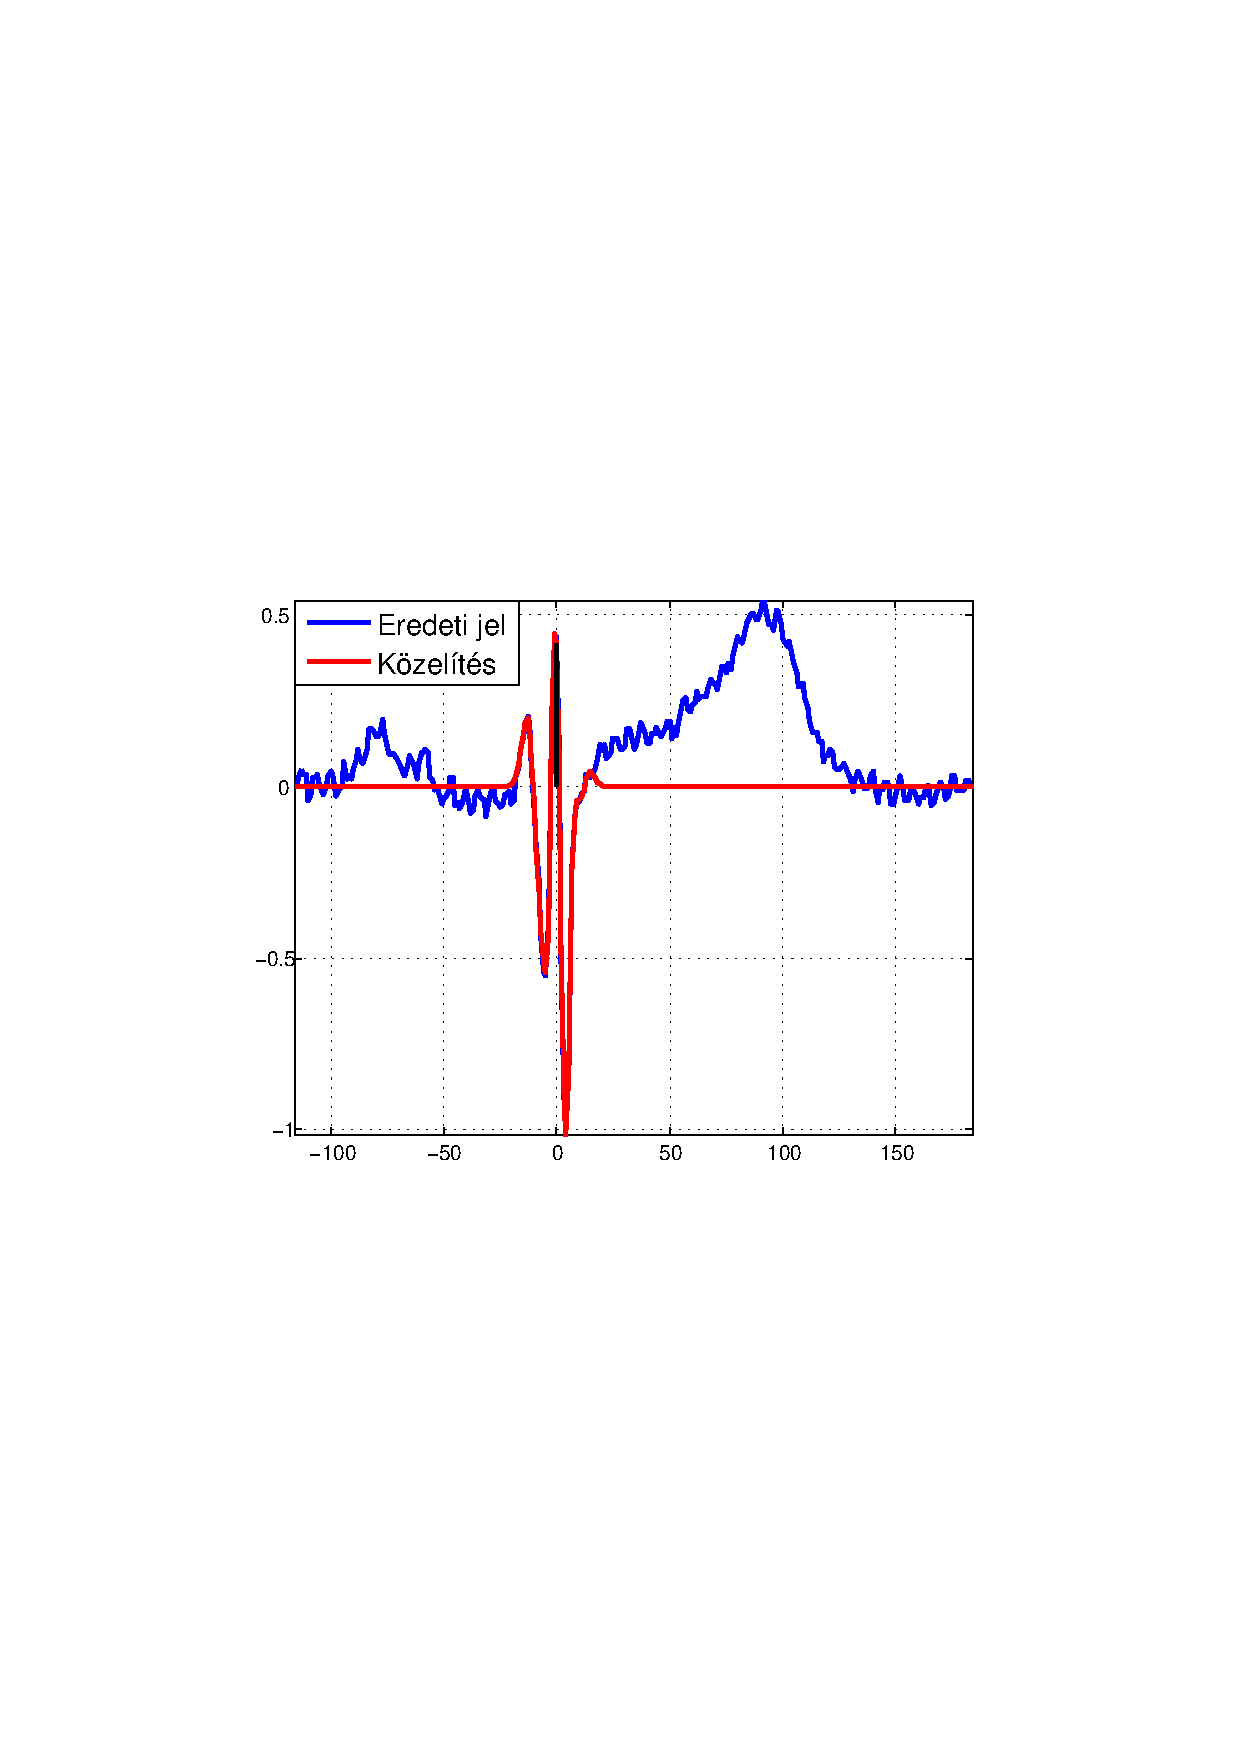
\includegraphics[scale=0.5,trim=120 280 100 280,clip]{./Abrak/Lepesek/abra_lepes0.pdf}} 
\subfigure[A T hullám approximációja.]{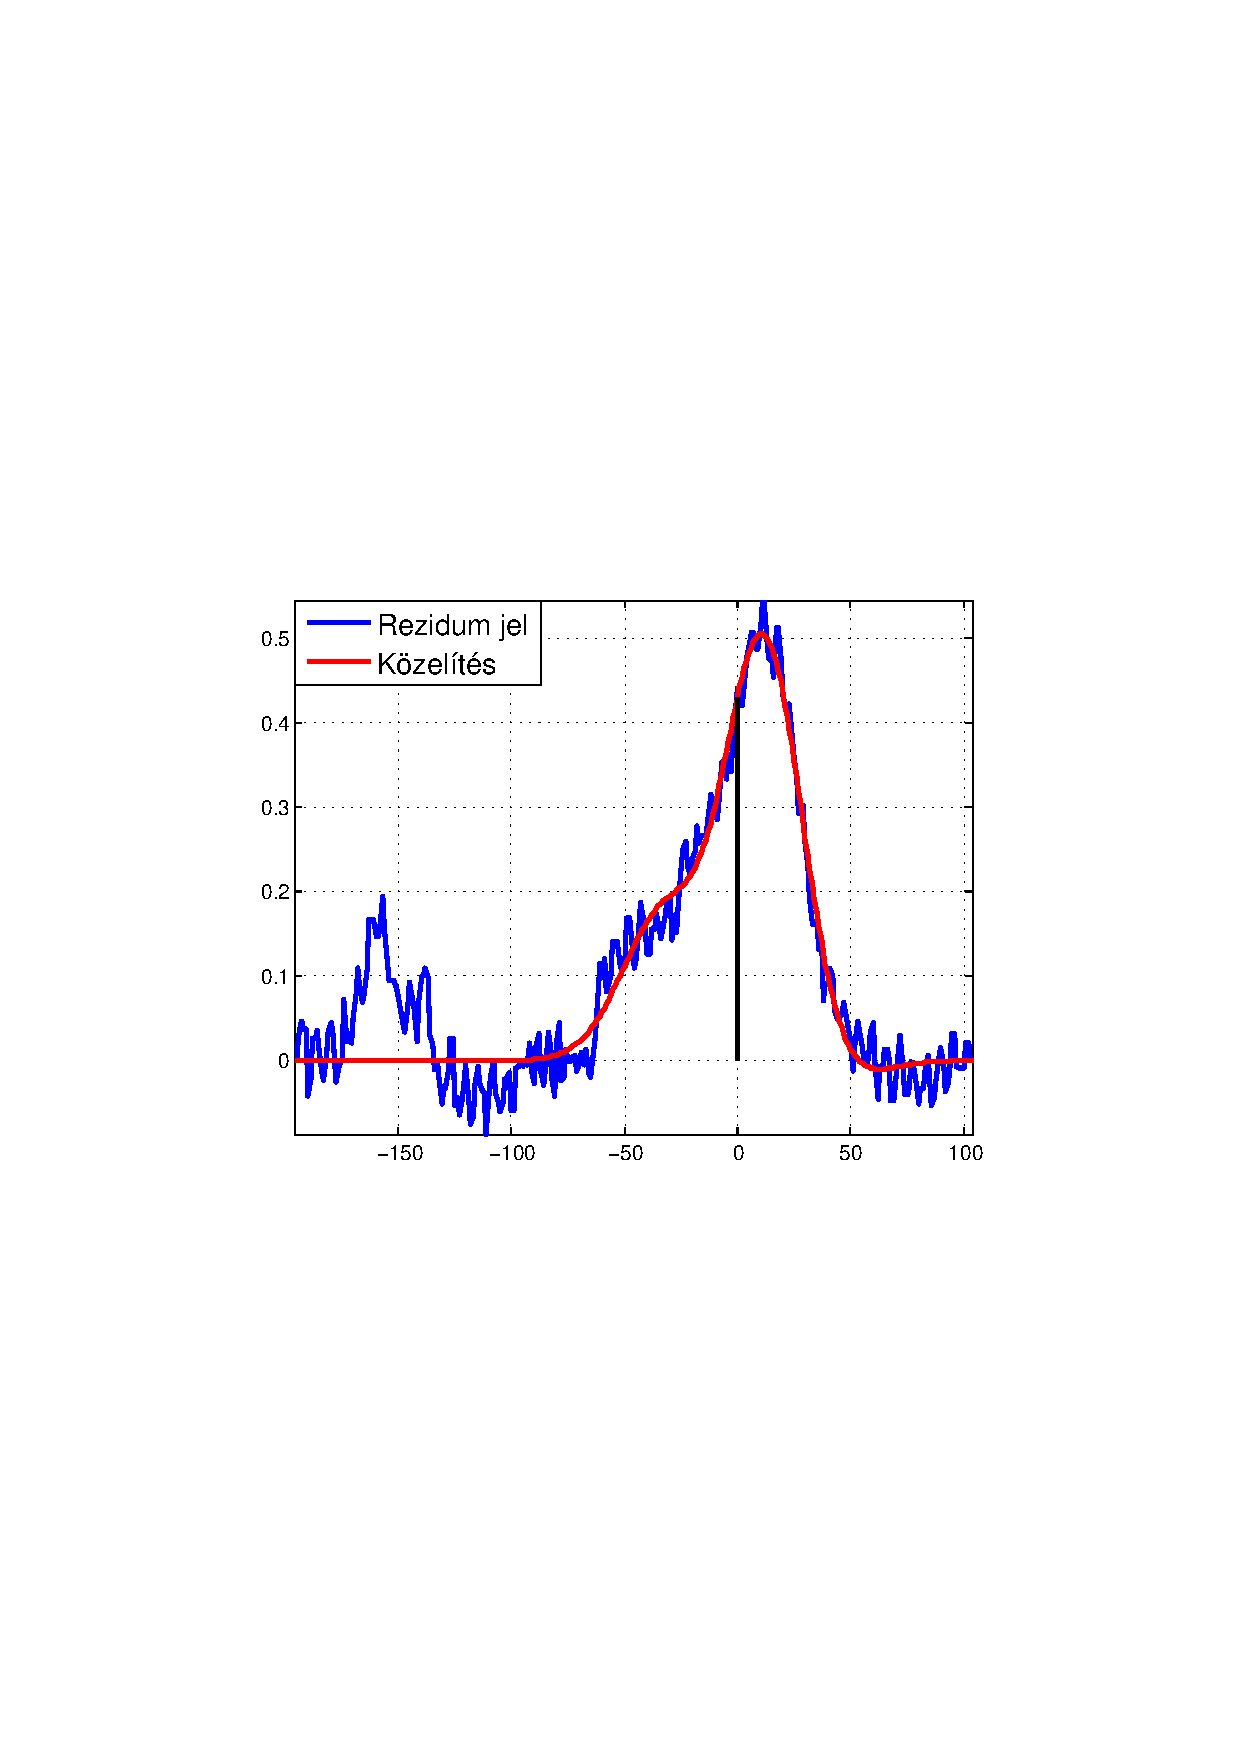
\includegraphics[scale=0.5,trim=120 280 100 280,clip]{./Abrak/Lepesek/abra_lepes1.pdf}}
\subfigure[A P hullám approximációja.]{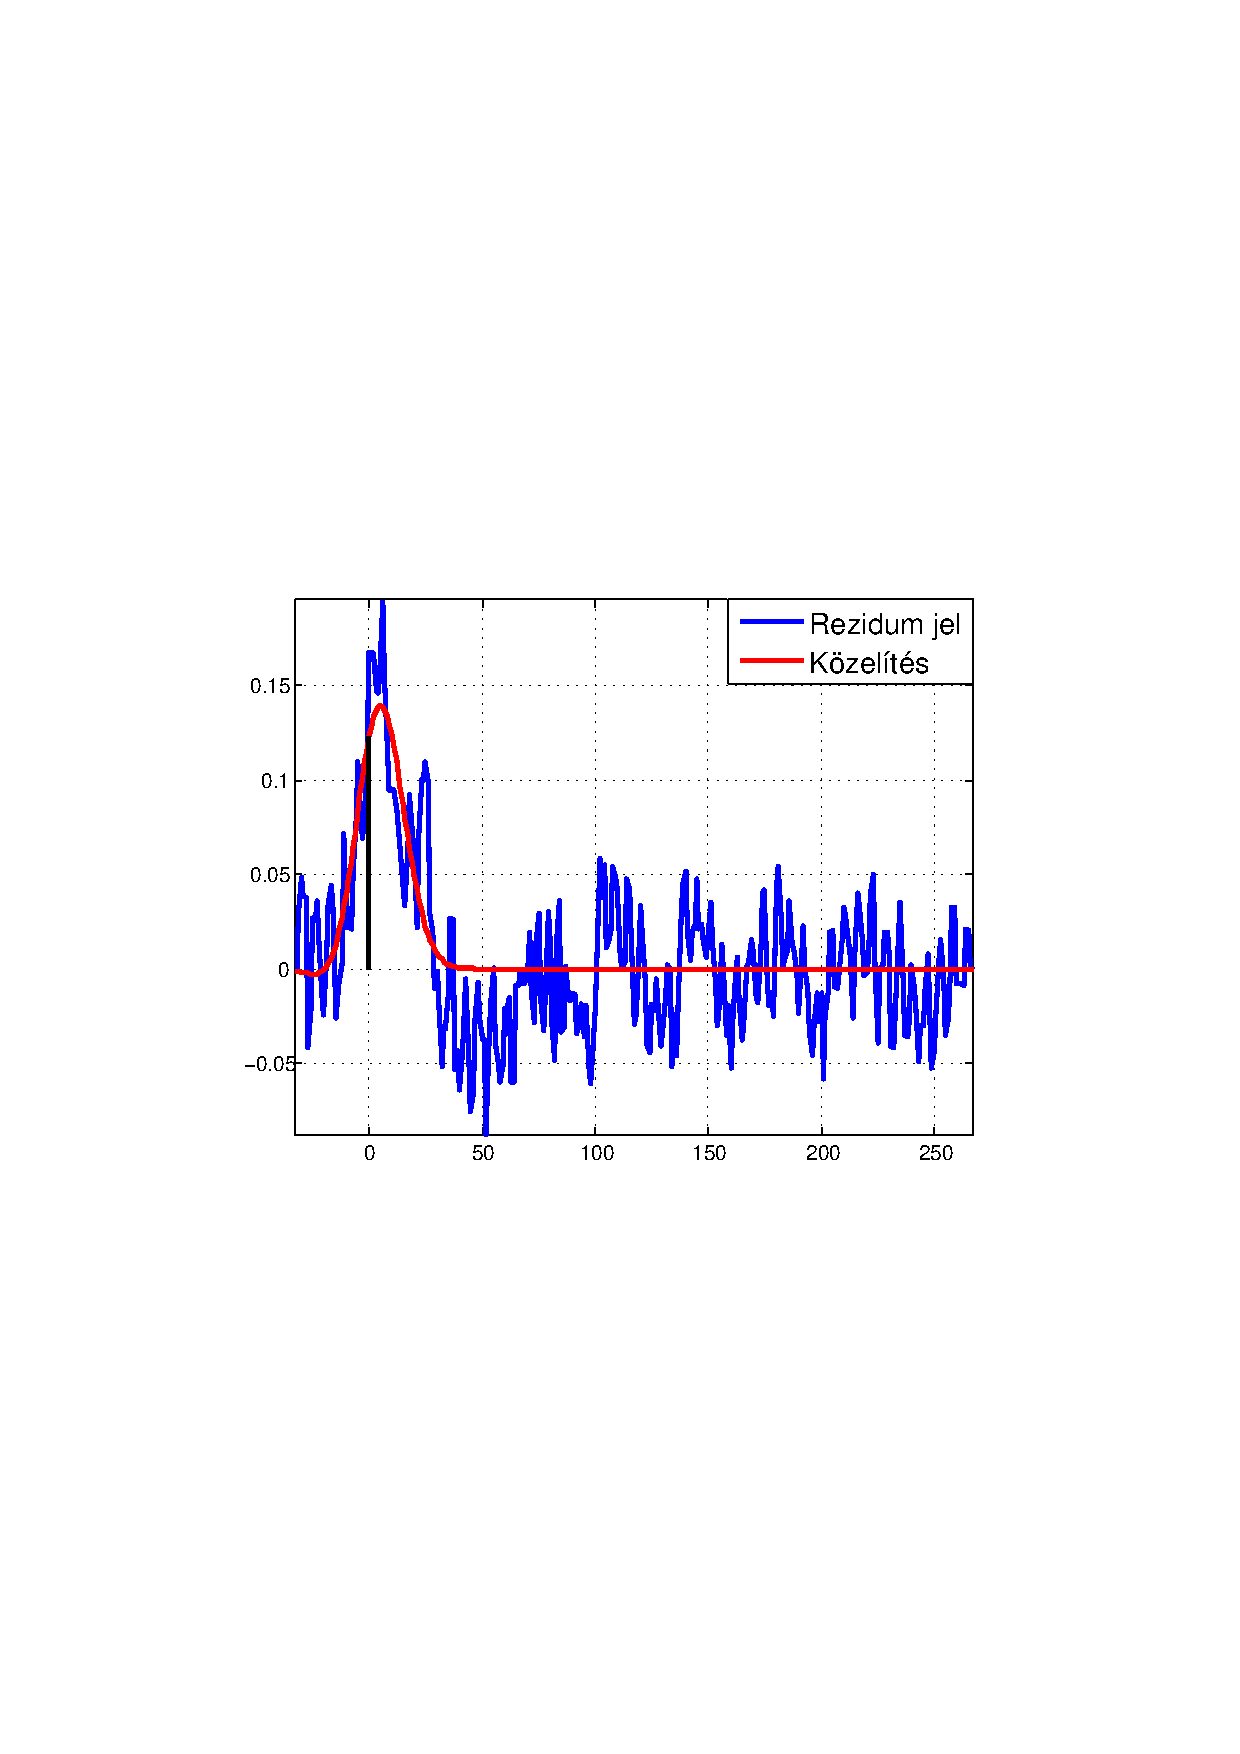
\includegraphics[scale=0.5,trim=120 280 100 280,clip]{./Abrak/Lepesek/abra_lepes2.pdf}} 
\subfigure[Szeparált szívütés.]{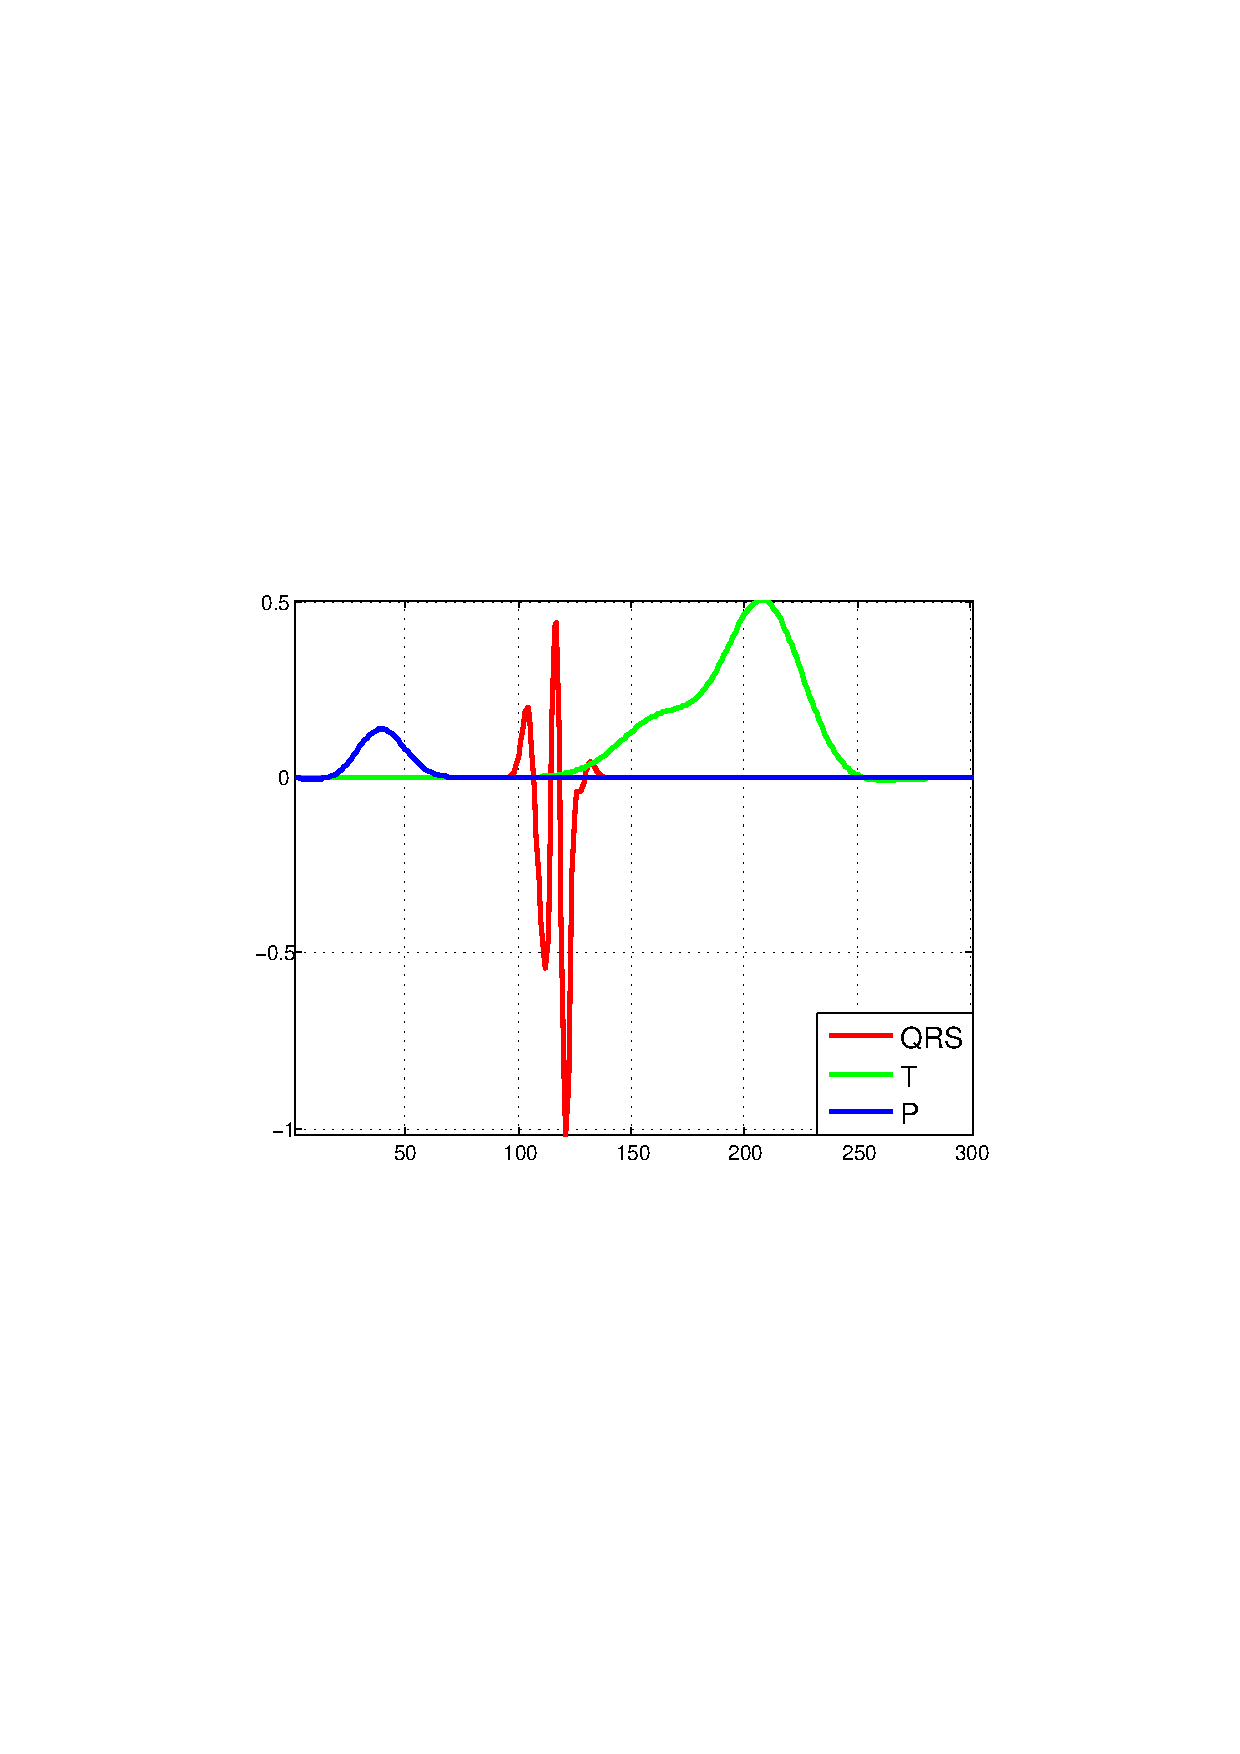
\includegraphics[scale=0.5,trim=120 280 100 280,clip]{./Abrak/Lepesek/abra_lepes3.pdf}}
\caption{Az MP algoritmus lépései.}
\label{fig:mpstep}
\end{figure}

\chapter{Felhasználói dokumentáció}

\chapter{Fejlesztői dokumentáció}

\end{document}
